
\chapter{Introduction}
\label{chapter_introduction}



%%%%%%%%%%%%%%%%%%%%%%%%%%%%%%%%%%%%%%%%%%%%%%%%%%%%%%%%%%%%

\section{Overview}


The continued increase of computing resources available for scientific and industrial research has motivated the simulation of complex flows. Several attempts have been done in order to fully simulate water-related hazards, from the generation up to their interaction with structures.

Usually, water-related hazards involve floods, which are complex natural phenomena with a great assortment of causes and a huge casuistic depending on the land characteristics or the climatic conditions. Preventing floods is still a great challenge due to uncertainty of climatic conditions and complexity of modeling land, usually defined by a great number of variables and parameters.

Furthermore, it is possible to identify several scales, local and global, with the local scale requiring a high fidelity simulation. The presence of such different levels of resolution makes the global simulation of these phenomena still unaffordable. Firstly, the event generation can be global or local. If it is local, a \emph{Fluid-Structure Interaction} (FSI) simulation may be needed. Then the propagation of the event usually allows to assume several simplifications, corresponding to the large scale field. Finally, the interaction with structures is strictly a local scale problem.

\emph{Landslide-Generated Waves} (LGW) are an example of water-related natural hazards. These events are originated when a landslide impacts a water reservoir and produces large-amplitude waves. LGW events can have devastating effects on the coastal areas of water basins, such as lakes, fjords and artificial reservoirs. Accurate modeling and prediction of LGWs are of key importance to reduce their catastrophic effects. Both experimental and numerical studies have greatly contributed to the enhancement of the forecasting capabilities against these natural hazards. In that case, both the generation of the impulse wave and the interaction with structures require a local-scale resolution.

The direct simulation of all the scenario with a local scale resolution is computationally highly demanding and it can become unaffordable as the size of the scenario increases. This fact leads to the consideration of alternative strategies combining the numerical simulation of the large and local scale in a staggered frame. Figure \ref{space_time_staggered_approach} shows a conceptual identification of the different scales and the possible approaches. The computational cost is proportional to the area enclosed by the space-time domain and proportional to the efficiency of each solver. In Figure \ref{space_time_staggered_approach} the local-scale resolution is identified with a \emph{Near Field Solver} (NFS) and the large-scale resolution is identified with a \emph{Far Field Solver} (FFS).

The staggered approach, apart from being less computationally intense, allows to decouple the uncertainty related to the generation of the event from the FSI simulation. In addition, the staggered approach allows to concentrate the computational resources only where they are needed, thus leading to a more efficient level of accuracy.


\begin{figure}
    \centering
    \includegraphics[width=\textwidth]{img/coupling/space_time}
    \caption{Propagation path of the event and possible computational approaches. Left: Brute force approach. Right: Staggered approach.}
    \label{space_time_staggered_approach}
\end{figure}


The main aspects that have been explored in this thesis are the numerical approximation of the FFS and the coupling strategy of the proposed FFS with an existing NFS. Special attention have been paid to the convergence and stability properties of the FFS aimed to solve the large scale.




%%%%%%%%%%%%%%%%%%%%%%%%%%%%%%%%%%%%%%%%%%%%%%%%%%%%%%%%%%%%

\section{Objectives and outline}


The work developed within the framework of this thesis can be enclosed in the global objective of investigating Finite Element formulations applied to large-scale water-related hazards. In particular, the analyzed methods have to be capable of reproducing local-scale effects around structures of interest and accurately model the large-scale propagation. This requirement lead to the analysis of the Finite Element Method for solving the Navier-Stokes equations on local scales and solving the shallow water equations on large scales.

The Navier-Stokes equations are typically solved using the finite element method, while the shallow water equations are often solved using the finite volume method.
Since we are interested in solving the global simulation within the same framework, a previous investigation on stabilized finite elements for the shallow water equations is presented.


This thesis is structured in 6 chapters, including the present introduction and a bibliographic revision. The bibliographic revision is specially extensive for the shallow water equations.
Chapter \ref{equations} presents a review of the governing equations which will be solved in the latter chapters.

Chapter \ref{eulerian_sw} is dedicated to the Finite Element Method applied to the shallow water equations. Stabilized formulations and quasi-monotonic formulations are presented.
Part of the developments of the numerical methods for the shallow water equations are moved to appendices \ref{lagrangian_sw} and \ref{mesh_refinement}, where the particle methods and mesh refinement are explored.
%This family of methods present some interesting properties, such as the natural approximation of the shoreline. The inconvenient of the Particle methods is the lack of robustness for all the possible flow regimes.

An extension of the shallow water equations to wave propagation on intermediate and deep water is presented in chapter \ref{eulerian_bsq}. These equations are known as the Boussinesq equations. The strategies developed in the previous chapter are applied to the Boussinesq equations, however, additional requirements must be fulfilled in order to ensure stability and accuracy. This chapter is of crucial importance in order to analyze impulse waves in the context of water-related hazards.

Chapter \ref{coupling} is devoted to the coupling strategies between the shallow water approximations --specially the Boussinesq equations-- and the fully resolved methods. An example of coupling for landslide long wave generation is provided.

Finally, the thesis is closed with some conclusions and possible further research lines in chapter \ref{conclusions}.


%%%%%%%%%%%%%%%%%%%%%%%%%%%%%%%%%%%%%%%%%%%%%%%%%%%%%%%%%%%%


\section{State of the art}
\label{state_art}


In this section a bibliographic revision of the methods employed to solve free surface flows problems is presented.
The general motion of a fluid is described by the Navier-Stokes equations. When free-surface water flows are considered, there are two implications, the incompressibility and homogeneous continuum medium enclosed by the interface. After presenting the most common numerical methods used to approximate the incompressible Navier-Stokes equations for free surface flows, the bibliographic review will be focused on the shallow water equations.
The shallow water equations are derived from the Navier-Stokes equations when some simplifications are assumed.
Finally, the bibliographic revision is closed with the coupling strategies for both models.



\subsection{Numerical methods for the Navier-Stokes model}


Nowadays, the accurate approximation of the fluid flow equations is aimed to represent the flow up to the smallest scales. In that sense, the effort is focused either on obtaining higher precision numerical schemes or in refining the discretization. The first approach is cheaper in contrast to the refinement approach, but the refinement approach have been proven to be much versatile. Even more, it is usually restrained to simple domain geometries. In the case of complex geometries, higher order approximations are equivalent to the \emph{Finite Volume methods} (FV) or \emph{Finite Element Methods} (FEM).

Nevertheless, when the Galerkin discretization is used within the frame of the FEM, an unstable behavior might appear. These instabilities are related to the non symmetric convection operator and to interpolation \cite{brezzi1991,codina2008oseen}. The stabilized methods like the \emph{Streamline Upwind Petrov Galerkin} (SUPG) \cite{hughes1986iii,brooks1982} can be framed in the \emph{Variational Multi-Scale} (VMS) concept \cite{hughes1995}. Latter, other stabilizations were presented, such as \emph{Finite-Increment Calculus} (FIC) \cite{onate1998} or \emph{Galerkin Least Squares} (GLS) \cite{hughes1989}. In fact, those stabilizations are of the same family of the previous ones, which consist on adding extra terms based on the residual of the balance equations. Since these stabilization techniques are consistent, allow for using higher order approximations.

However, the number of terms introduced by stabilizations in order to keep consistency notably increase, can couple unknowns and increase the non-symmetry of the system. In order to overcome this issues, projection methods only introduce the terms required for stability purpose. The key of these methods is the choice of the projector. A global $L^2$ projector is used in the orthogonal sub scales method \cite{codina2000}. Other methods avoiding the global projection are named local projection stabilization \cite{braack2006,matthies2007} or nodal projection stabilization \cite{badia2012}.


Apart from the stabilization technique for the Navier-Stokes equations, the numerical approximation must be able to deal with the interface discontinuity. Concerning the coordinate frame where the governing equations are solved, the solution methods can be classified in Eulerian and Lagrangian formulations. Classical numerical methods to solve CFD problems typically use the Eulerian formulation with a level set function \cite{chen1997} with enriched shape functions \cite{burman2015cut}. Very often, Lagrangian formulations take advantage on the possibility of the FEM to discretize complex geometries. In that case, the FEM is combined with a mesh moving and remeshing strategy. It can be applied in an \emph{Arbitrary Lagrangian-Eulerian formulation} (ALE) \cite{donea2004} or in a pure Lagrangian formulation. This is the case of the \emph{Particle Finite Element Method} (PFEM) \cite{onate2004,idelsohn2004}

Regardless the framework where the governing equations are solved, the formulation needs to be stabilized in order to fulfill the \emph{inf-sup} condition \cite{brezzi1991}. In this work, the PFEM formulation stabilized with FIC will be used. It has been successfully applied to solve free surface flows \cite{delpin2007} and FSI analysis \cite{onate2008} or in combination with other numerical models \cite{onate2022}.


\subsection{Numerical methods for the shallow water models}


When large scale free surface flows are considered, some simplifications can be assumed, such as small vertical scale and hydrostatic pressure distribution. These assumptions allow to express the Navier-Stokes equations in a depth averaged balance, which are the shallow water equations. Depending on the assumptions, slightly different equations are obtained. While the Saint-Venant equations are well suited for convective flows, the Boussinesq equations describe the oscillatory phenomena of waves. Anyway, both systems of equations are hyperbolic and present an analogy with the Euler conservation laws or compressible Navier-Stokes equations. Hence, the numerical methods commonly used for the compressible Navier-Stokes equations can be applied to the shallow water equations.

The novelty of the shallow water equations with respect to the Navier-Stokes equations is the fact that the domain is restricted to the wet area. The wet area is described by the positive water depth, there where the depth integration is defined. The shoreline moves according to the dynamics and is characterized by a null water depth, a region where the equations are singular and the system is no longer hyperbolic. This property will need specific numerical considerations.

Löhner \cite{lohner2008} made a review of possible approximation methods to solve fluid dynamics. Being a discretization $u^h = N^i\hat{u}_i$ ($i=1,2,\dots,m$) approximating the solution $u$, the weighted residual is defined as
\begin{equation*}
\int_{\Omega} W^ir(u^h)d\Omega = 0
\end{equation*}
This description allows to wrap the most common numerical methods in the same frame. Depending on the choice of the basis functions $N$ and the trial function $W$, the weighted residual yields several numerical methods. Table \ref{possible_trial_functions} summarizes the most common choices of trial functions.

\begin{table}
\centering
\begin{tabular}{|l|c|c|}
\hline
 & $N^i$ & $W^i$ \\ \hline
Finite differences (FD)         & polynomial & $\delta(x_i)$ \\ \hline
Finite volumes (FV)             & polynomial & $1 \ \text{if} \ x\in\Omega_{el}$ \\ \hline
Galerkin finite elements (FEM)  & polynomial & $N^i$ \\ \hline
Discontinuous Galerkin (DG)     & polynomial & $N^i \ \text{if} \ x\in\Omega_{el}$ \\ \hline
\end{tabular}
\caption{Possible choices of trial and test functions $N^i$ and $W^i$}
\label{possible_trial_functions}
\end{table}

The method most commonly used in the shallow water community are FV by its stability properties when dealing with the moving shoreline \cite{abbott1978,leveque2002}. More recently, the \emph{Discontinuous Galerkin} technique has been applied to the shallow water equations \cite{ambati2007,khan2014,lee2019}. Like FV, the DG method has the advantage of computing the fluxes at the element boundary, allowing the method to naturally consider the moving shoreline. However, the introduction of high order DG schemes is not straightforward.

In this research the FEM for the shallow water equations will be explored. Apart from its ability to solve the oscillatory problem of the Boussinesq equations, it will allow a unified formulation for the coupling strategy. When the FEM is considered, several sources of instabilities arise. Firstly, the \emph{inf-sup} condition if the same space of interpolation is used for all the variables. Secondly, analogously to compressible flows, shocks might appear in the regime variations, from sub-critical to super-critical. Lastly, Gibbs oscillations appear at the shoreline, since the partially wet elements are not able to preserve the water positivity.

The stabilized FEM are known to ensure global stabilization, however, monotonic properties are not inherited by the numerical scheme. Monotonicity is related to the Godunov barrier theorem \cite{godunov1959} where is stated that a scheme or order higher than 1 is not oscillatory free. The \emph{Flux Corrected Transport} FCT algorithm \cite{lohner2008ch9} uses the Godunov theorem to construct a non linear scheme which combines a low order non-oscillatory scheme with a high order one. The process of combining the two schemes is called limiting.

Other methods inspired in the flux limiting are the edge based schemes \cite{lohner2008ch10}. The edge based structure is an efficient way to assemble the system matrix which resort to a FV approximation of convective terms. If it is assumed that the fluxes of the variables are constant along the edges, a discontinuity will occur at the edge midpoint. Then, one can replace the Galerkin flux by a Riemann flux and obtain a \emph{Total Variational Diminishing} scheme (TVD).

Finally, non-linear stabilizations are a more consistent way to add local stabilizations around shocks and the moving shoreline \cite{codina2011}. Badia and Hierro presented a monotonicity preserving stabilized finite element for hyperbolic equations \cite{badia2014}.



\subsection{Coupling strategies}


Accurate modeling and prediction of LGWs are of key importance to reduce their catastrophic effects.
Both experimental and numerical studies have been greatly contributed to the enhancement of the forecasting capabilities against these natural hazards.

Physical models are particularly helpful to identify the key parameters of both the sliding material and the water body and to determine their specific effect on the LGW scenario \cite{noda1970water, fritz2004near, heller2011wave, mohammed2012physical, romano2016, mulligan2017, evers2019spatial}. A detailed overview of experimental tests applied to LGW events can be found in \cite{yavari2017subaerial}. Nevertheless, laboratory tests are mainly devoted to determining the near-field wave conditions, while estimations on the far-field waves, which are responsible for major damages to the coastal areas affected by an LGW event, are more difficult to extrapolate.

On the other hand, numerical methods have the potential to predict both near- and far-field waves characteristics. However, the numerical simulation of a LGW is a challenging task. Indeed, the computational method must be able to model the complex constitutive behavior of the landslide material, deal with fluid-solid (or multi-fluid) interaction, and track the largely evolving topology of both landslide and water bodies. Furthermore, the LGW analysis involves different characteristic time and space scales for the near field (landslide-water impact zone) and the far field (wave propagation). Finally, it is required to solve large-scale three-dimensional (3D) geometries for long time durations, and this makes the computational cost of LGW analyses one of the most critical issues.

The numerical models applied to LGWs can be classified into three main groups \cite{yavari2016numerical} briefly summarized below.

The first approach consists in using a wave propagation solver, typically based on Shallow Water (SW) equations. In this strategy, the landslide runout and water impact are not resolved but are introduced into the model as an equivalent boundary condition \cite{waythomas2003numerical, ataie2008mapping}. This approach is the simplest one and has the lowest computational cost. However, it assumes strong simplifications on both the landslide motion and momentum transfer and thus it can only give an approximate idea of the global LGW scenario.

In the second strategy, the landslide and water motion equations are solved in a unique coupled model. First applications of this holistic strategy can be found in \cite{kelfoun2010landslide} and \cite{giachetti2011numerical}, where shallow water models were used for both the landslide and the water body.
Only recently, more accurate 3D monolithic approaches for LGW problems have been presented, see for example
\cite{vacondio20133d, CrostaVajont, franci20203dA, franci20203dB, xu2021sph, terada2021}. Nevertheless, the computational cost of this fully resolved method can be still unaffordable for large-scale events.

The third approach splits the LGW problem into two simulations that interact with each other at their interface. Typically, in these so-called partitioned strategies, a numerical method, here called $near$-$field$ $solver$ (NFS), computes the landslide runout, impact against the water body and wave formation. A different numerical scheme, here called $far$-$field$ $solver$ (FFS), predicts the far-field wave propagation \cite{yavari2016numerical}.
Generally, a weak (or one-way) coupling scheme is adopted, meaning that the NFS is insensitive to the FFS solution. The one-way coupling simplification preserves the computational advantages of this partitioned approach and it still ensures an accurate modeling of the key phenomena of an LGW scenario, such as the landslide runout, the wave generation and the far-field wave propagation.
%In order to keep the computational advantages of this partitioned approach, a weak (or one-way) coupling scheme is generally adopted, meaning that the NFS is insensitive to the FFS solution. The one-way coupling simplification has a negligible effect both on the water wave generation and on the far-field wave propagation and runup, which are the key phenomena of an LGW scenario.
 
One of the first applications of this partitioned method for LGWs was presented in \cite{heinrich1998simulation}. In this work, a simplified 3D model was used for the landslide-water impact and a shallow water model was applied for the far-field wave propagation.
In \cite{lovholt2008oceanic}, a potential tsunami scenario induced by the collapse of a part of Cumbre Vieja Volcano of La Palma island, Spain, was studied by coupling a 3D compressible Eulerian solver with a Boussinesq model. In \cite{abadie2012numerical}, the same case study was analyzed using a 3D Volume Of Fluid (VOF) method, as the NFS, and an analogous FFS such as that used in \cite{lovholt2008oceanic}.
More recently, Tan et al. \cite{tan2018numerical} coupled a Smoothed Particle Hydrodynamics (SPH) method with a shallow water equations solver was used to reproduce hypothetical LGW scenarios at Es Vedrà, Ibiza, Spain.

%In this work, we propose and validate a novel partitioned model for LGWs. In this new strategy, a Lagrangian finite element method, namely the Particle Finite Element Method (PFEM) \cite{PFEM2004, onate2004, cremonesi2020state}, is used as the NFS and a standard shallow water Boussinesq model is used as the FFS. Several previous works have shown the accuracy of the PFEM to model landslides \cite{PFEMzhang1, PFEMzhangLandslide, zhang2021gpu}, also in cascading events \cite{CremonesiPFEM2, Salazar2012, CremonesiSlipLandslides, ZhangSubmarine}. In this work, we use the PFEM approach that has been successfully applied to LGW scenarios in \cite{mulligan2020} and in \cite{franci20203dA, franci20203dB}, where 3D simulations of the Vajont disaster were presented. 
%This work aims at being a proof of concept of this new coupled strategy for real LGW scenarios. For this reason, a deep validation of the method is presented by analyzing the performance and accuracy of the new partitioned technique in targeted tests, using reference solutions obtained with other numerical methods, experimental tests and analytical solutions.
%In partitioned methods, the momentum transfer between the Navier-Stokes and the Boussinesq models must be accurate in order to obtain a faithful representation of the LGW scenario. Thus, particular attention is devoted here to analyze the effect of the near-field boundary conditions on the far-field propagating wave. Convergence and sensitivity analyses are carried out in order to verify the accuracy and robustness of the proposed method. 






%%%%%%%%%%%%%%%%%%%%%%%%%%%%%%%%%%%%%%%%%%%%%%%%%%%%%%%%%%%%

\section{Research dissemination}


Some of the developments if this thesis have been published in the format of articles in peer reviewed journals. Since the research has advanced gradually, the articles are related to a chapter, but there are some differences, which can be big.
The chapters are more extensive than the articles and some parts of the articles are omitted to avoid repetitions.
There is also not the same sequence between the publication date and the chapter order.
On the other hand, since the notation is introduced gradually, it has been unified in the thesis and may be slightly different from the articles and this document.

\paragraph{Chapter \ref{eulerian_sw}} \fullcite{maso2022}
\paragraph{Chapter \ref{coupling}} \fullcite{maso2022b} (preprint)
\paragraph{Appendix \ref{lagrangian_sw}} \fullcite{puigferrat2021}
\\

In addition, the content of the chapters has been also disseminated in the form of oral presentations in scientific conferences and congresses:

\paragraph{Chapter \ref{coupling}} \fullcite{wccm2022} (Abstract accepted)
\paragraph{Chapter \ref{coupling}} \fullcite{cmn2022} (Abstract accepted)
\paragraph{Chapter \ref{coupling}} \fullcite{eccomas2022}
\paragraph{Appendix \ref{lagrangian_sw}} \fullcite{particles2019}

